% Abel Prize — Laureates (2003–2026)
% Compact tabular layout mirroring fields_medal_laureates_beamer.tex
% Cross-award badges per math_awards_allinone.tex
% Compile with: xelatex abel_prize_laureates_beamer.tex

\documentclass[aspectratio=169,9pt]{beamer}

% ---- Theme ----
\usetheme{default}
\usecolortheme{default}
\setbeamertemplate{navigation symbols}{}
\setbeamertemplate{footline}{%
  \hfill{\tiny\color{mutedgray}\insertframenumber/\inserttotalframenumber}\hspace*{6pt}\vspace{4pt}%
}
\newcommand{\framesubject}{}
\setbeamertemplate{frametitle}{%
  \vspace{8pt}%
  \centering
  {\large\bfseries\color{abelclr}阿贝尔奖 \insertframetitle}\\[3pt]
  {\footnotesize\color{mutedgray}\framesubject}\\[4pt]
  \textcolor{abelbg}{\rule{0.95\textwidth}{0.6pt}}%
  \vspace{-6pt}%
}

% ---- Fonts & Language ----
\usepackage{fontspec}
\usepackage{xeCJK}
\setCJKmainfont{PingFang SC}[BoldFont=PingFang SC Semibold]
\setCJKsansfont{PingFang SC}
\setmainfont{Helvetica Neue}[BoldFont=Helvetica Neue Bold]
\setsansfont{Helvetica Neue}

% ---- Packages ----
\usepackage{booktabs}
\usepackage{array}
\usepackage{tikz}
\usepackage{amssymb}
\usepackage{colortbl}
\usepackage{graphicx}\usepackage{fontawesome5}

% ---- Colors ----
\definecolor{headerblue}{RGB}{41,65,122}
\definecolor{yearcolor}{RGB}{150,40,90}
\definecolor{fieldcolor}{RGB}{30,100,60}
\definecolor{mutedgray}{RGB}{100,100,100}
\definecolor{slidebg}{RGB}{255,250,252}
% ---- Per-award brand colors (match math_awards_allinone) ----
\definecolor{fieldsclr}{RGB}{41,65,122}   % Fields — 深蓝
\definecolor{wolfclr}{RGB}{150,100,0}
\definecolor{coverprimary}{HTML}{1A56DB}
\definecolor{nobelclr}{RGB}{176,141,45}   % Nobel Economics — gold
    % Wolf   — 金棕
\definecolor{abelclr}{RGB}{150,40,90}     % Abel   — 紫红（主色）
\definecolor{chernclr}{RGB}{15,110,92}    % Chern  — 翡翠绿
\definecolor{abelbg}{RGB}{238,218,228}    % 表头底色
\definecolor{fieldsbg}{RGB}{230,235,250}  % Fields 浅蓝底
\definecolor{wolfbg}{RGB}{252,245,230}    % Wolf 浅金底
\definecolor{chernbg}{RGB}{225,245,238}   % Chern 浅绿底
\definecolor{nobelbg}{RGB}{252,246,228}   % Nobel 浅金底
\definecolor{turingbg}{RGB}{225,235,252}  % Turing 浅蓝底

% ---- Beamer Colors ----
\setbeamercolor{background canvas}{bg=slidebg}
\setbeamercolor{title}{fg=abelclr}

% ---- Custom Commands ----
% 奖项徽标：追加在姓名后，标注该得主还获得的其他顶级奖项
\newcommand{\fieldsbadge}{\textsuperscript{\normalfont\tiny\color{fieldsclr}$\blacklozenge$\kern-0.5pt F}}
\newcommand{\wolfbadge}{\textsuperscript{\normalfont\tiny\color{wolfclr}$\bigstar$\kern-0.5pt W}}
\newcommand{\chernbadge}{\textsuperscript{\normalfont\tiny\color{chernclr}$\blacksquare$\kern-0.5pt C}}
\newcommand{\nobelbadge}{\textsuperscript{\normalfont\tiny\color{nobelclr}\faIcon{award}\kern-0.5pt N}}
\newcommand{\turingbadge}{\textsuperscript{\normalfont\tiny\color{coverprimary}\faIcon{desktop}\kern-0.5pt T}}

% Table row for a laureate
% #1=Name(+badges), #2=Year, #3=Birth-Death, #4=Nationality, #5=Institution, #6=Field
% Name cell carries a \cn{中文名} suffix rendered on its own line in muted gray.
\newcommand{\cn}[1]{\newline{\scriptsize\color{mutedgray}#1}}
\newcommand{\lrow}[6]{%
  {\bfseries\color{abelclr}#1} & {\color{yearcolor}#2} & {#3} & {#4} & {\scriptsize #5} & {\scriptsize\color{fieldcolor}#6} \\[2.5pt]
}

% ---- Document ----
\begin{document}

% ============================================================
% Title Slide
% ============================================================
\begin{frame}[plain]
\begin{tikzpicture}[remember picture, overlay]
  \fill[abelclr!2] (current page.north west) rectangle (current page.south east);
  \fill[abelclr!6] (current page.north west) ++(1.55,-1.35) circle (2.45cm);
  \fill[abelclr!8] (current page.south east) ++(-1.9,1.45) circle (2.70cm);
  \node[anchor=center, font=\fontsize{18}{24}\selectfont\bfseries, text=abelclr]
    at ([yshift=2.80cm]current page.center) {阿贝尔奖：数学家的终身成就奖（2003–2026）};
  \node[anchor=center, font=\fontsize{11}{15}\selectfont, text=mutedgray]
    at ([yshift=1.60cm]current page.center) {Abel Prize\enspace·\enspace 数学界的诺贝尔奖\enspace·\enspace 全 29 位得主};
  \draw[abelclr!50, line width=1.2pt] ([yshift=0.90cm, xshift=-5.0cm]current page.center)
    -- ([yshift=0.90cm, xshift=5.0cm]current page.center);
  \node[anchor=center, font=\fontsize{9}{12}\selectfont\bfseries, text=mutedgray]
    at ([yshift=0.20cm]current page.center) {兼录菲尔兹·沃尔夫·陈省身·诺贝尔经济学·图灵奖双料·大满贯得主};
  \node[anchor=center] at ([yshift=-1.90cm]current page.center) {
    \begin{tikzpicture}[scale=1]
      % Row 1 (10): 2003–2010
      \node[inner sep=0pt] at (-5.00,0.85) {
        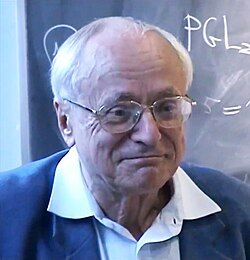
\includegraphics[width=1.05cm,height=1.30cm,keepaspectratio]{images/serre.jpg}
      };
      \node[inner sep=0pt] at (-3.89,0.85) {
        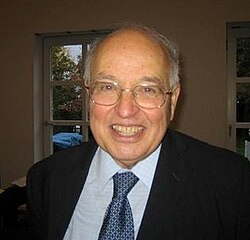
\includegraphics[width=1.05cm,height=1.30cm,keepaspectratio]{images/atiyah.jpg}
      };
      \node[inner sep=0pt] at (-2.78,0.85) {
        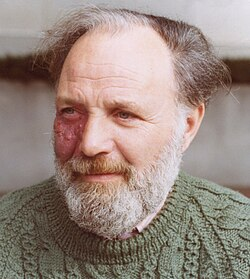
\includegraphics[width=1.05cm,height=1.30cm,keepaspectratio]{images/singer.jpg}
      };
      \node[inner sep=0pt] at (-1.67,0.85) {
        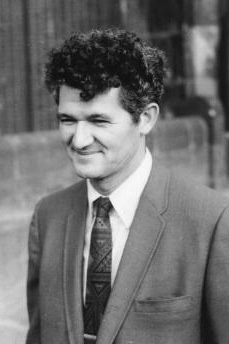
\includegraphics[width=1.05cm,height=1.30cm,keepaspectratio]{images/lax.jpg}
      };
      \node[inner sep=0pt] at (-0.56,0.85) {
        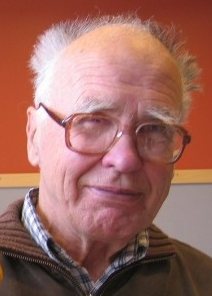
\includegraphics[width=1.05cm,height=1.30cm,keepaspectratio]{images/carleson.jpg}
      };
      \node[inner sep=0pt] at (0.56,0.85) {
        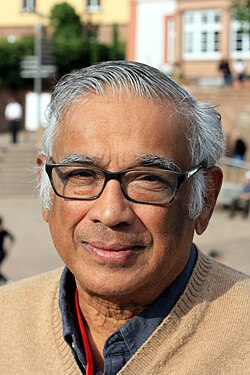
\includegraphics[width=1.05cm,height=1.30cm,keepaspectratio]{images/varadhan.jpg}
      };
      \node[inner sep=0pt] at (1.67,0.85) {
        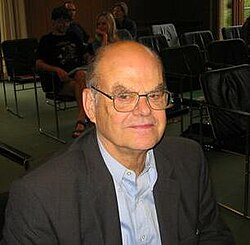
\includegraphics[width=1.05cm,height=1.30cm,keepaspectratio]{images/thompson.jpg}
      };
      \node[inner sep=0pt] at (2.78,0.85) {
        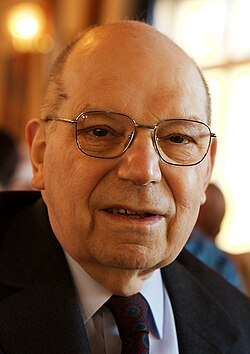
\includegraphics[width=1.05cm,height=1.30cm,keepaspectratio]{images/tits.jpg}
      };
      \node[inner sep=0pt] at (3.89,0.85) {
        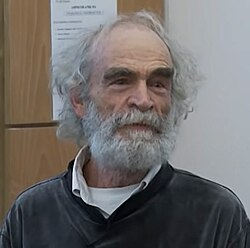
\includegraphics[width=1.05cm,height=1.30cm,keepaspectratio]{images/gromov.jpg}
      };
      \node[inner sep=0pt] at (5.00,0.85) {
        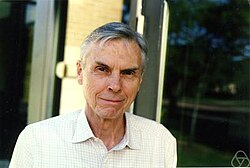
\includegraphics[width=1.05cm,height=1.30cm,keepaspectratio]{images/tate.jpg}
      };

      % Row 2 (10): 2011–2018
      \node[inner sep=0pt] at (-5.00,0.0) {
        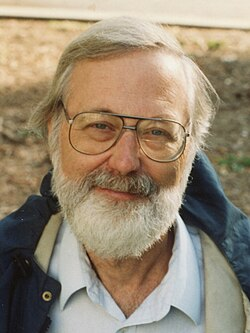
\includegraphics[width=1.05cm,height=1.30cm,keepaspectratio]{images/milnor.jpg}
      };
      \node[inner sep=0pt] at (-3.89,0.0) {
        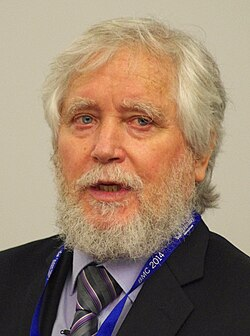
\includegraphics[width=1.05cm,height=1.30cm,keepaspectratio]{images/szemeredi.jpg}
      };
      \node[inner sep=0pt] at (-2.78,0.0) {
        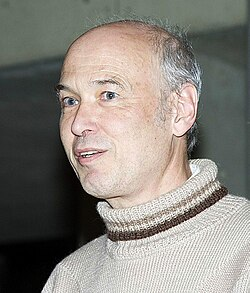
\includegraphics[width=1.05cm,height=1.30cm,keepaspectratio]{images/deligne.jpg}
      };
      \node[inner sep=0pt] at (-1.67,0.0) {
        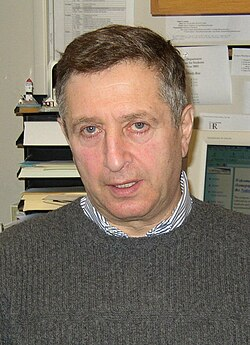
\includegraphics[width=1.05cm,height=1.30cm,keepaspectratio]{images/sinai.jpg}
      };
      \node[inner sep=0pt] at (-0.56,0.0) {
        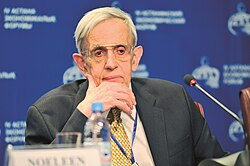
\includegraphics[width=1.05cm,height=1.30cm,keepaspectratio]{images/nash.jpg}
      };
      \node[inner sep=0pt] at (0.56,0.0) {
        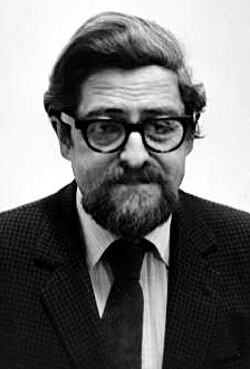
\includegraphics[width=1.05cm,height=1.30cm,keepaspectratio]{images/nirenberg.jpg}
      };
      \node[inner sep=0pt] at (1.67,0.0) {
        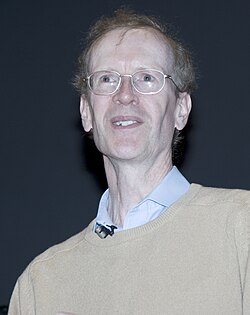
\includegraphics[width=1.05cm,height=1.30cm,keepaspectratio]{images/wiles.jpg}
      };
      \node[inner sep=0pt] at (2.78,0.0) {
        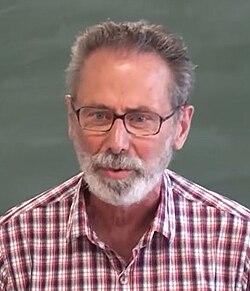
\includegraphics[width=1.05cm,height=1.30cm,keepaspectratio]{images/meyer.jpg}
      };
      \node[inner sep=0pt] at (3.89,0.0) {
        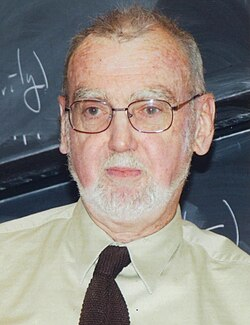
\includegraphics[width=1.05cm,height=1.30cm,keepaspectratio]{images/langlands.jpg}
      };
      \node[inner sep=0pt] at (5.00,0.0) {
        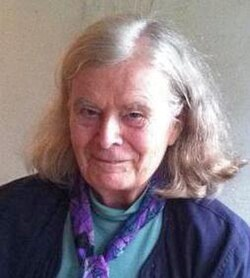
\includegraphics[width=1.05cm,height=1.30cm,keepaspectratio]{images/uhlenbeck.jpg}
      };

      % Row 3 (9): 2020–2026
      \node[inner sep=0pt] at (-5.00,-0.85) {
        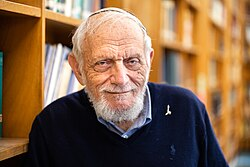
\includegraphics[width=1.05cm,height=1.30cm,keepaspectratio]{images/furstenberg.jpg}
      };
      \node[inner sep=0pt] at (-3.75,-0.85) {
        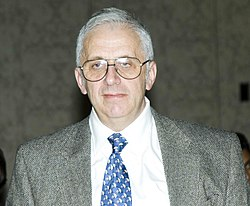
\includegraphics[width=1.05cm,height=1.30cm,keepaspectratio]{images/margulis.jpg}
      };
      \node[inner sep=0pt] at (-2.50,-0.85) {
        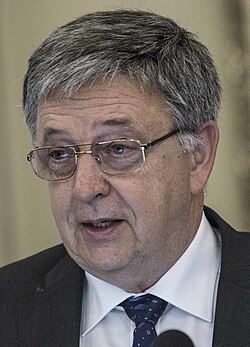
\includegraphics[width=1.05cm,height=1.30cm,keepaspectratio]{images/lovasz.jpg}
      };
      \node[inner sep=0pt] at (-1.25,-0.85) {
        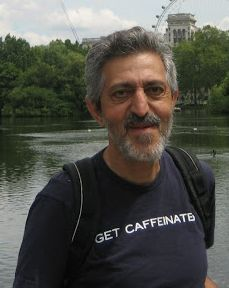
\includegraphics[width=1.05cm,height=1.30cm,keepaspectratio]{images/wigderson.jpg}
      };
      \node[inner sep=0pt] at (0.00,-0.85) {
        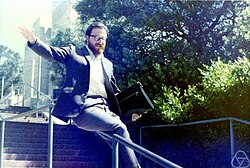
\includegraphics[width=1.05cm,height=1.30cm,keepaspectratio]{images/sullivan.jpg}
      };
      \node[inner sep=0pt] at (1.25,-0.85) {
        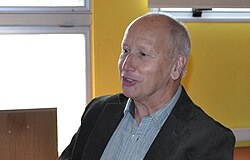
\includegraphics[width=1.05cm,height=1.30cm,keepaspectratio]{images/caffarelli.jpg}
      };
      \node[inner sep=0pt] at (2.50,-0.85) {
        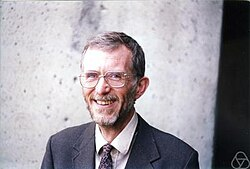
\includegraphics[width=1.05cm,height=1.30cm,keepaspectratio]{images/talagrand.jpg}
      };
      \node[inner sep=0pt] at (3.75,-0.85) {
        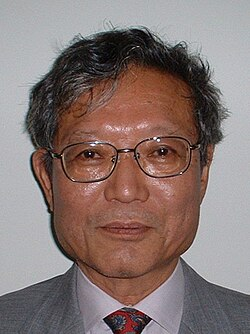
\includegraphics[width=1.05cm,height=1.30cm,keepaspectratio]{images/kashiwara.jpg}
      };
      \node[inner sep=0pt] at (5.00,-0.85) {
        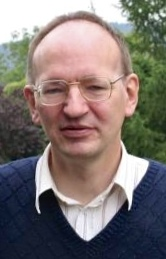
\includegraphics[width=1.05cm,height=1.30cm,keepaspectratio]{images/faltings.jpg}
      };
    \end{tikzpicture}
  };
  \node[anchor=south, font=\fontsize{6}{7}\selectfont, text=mutedgray]
    at ([yshift=0.38cm]current page.south) {\faIcon{medal}\enspace Abel Prize Laureates\enspace|\enspace 挪威科学与文学院\enspace|\enspace 2003–2026};
\end{tikzpicture}
\end{frame}


% Table slide 1: 2003–2006
\def\framesubject{拓扑·代数几何·数论}
\begin{frame}{2003–2006}
\vspace{-2pt}
\centering
\scriptsize
\begin{tabular}{@{}
  >{\raggedright}m{3.6cm}
  >{\centering}m{0.95cm}
  >{\centering}m{1.05cm}
  >{\raggedright}m{1.5cm}
  >{\raggedright}m{2.4cm}
  >{\raggedright\arraybackslash}m{2.6cm}
@{}}
\toprule
\rowcolor{abelbg}
\textbf{姓名} & \textbf{年份} & \textbf{生卒} & \textbf{国籍} & \textbf{机构} & \textbf{研究领域} \\
\midrule
\lrow{Jean-Pierre Serre\fieldsbadge\wolfbadge\cn{让-皮埃尔·塞尔}}{2003}{1926–}{法国}{Collège de France}{拓扑、代数几何、数论；亦获 F1954 / W2000}
\lrow{Michael Atiyah\fieldsbadge\cn{迈克尔·阿蒂亚}}{2004}{1929–2019}{英国}{Univ. of Edinburgh}{Atiyah–Singer 指标定理；亦获 F1966}
\lrow{Isadore Singer\cn{伊萨多·辛格}}{2004}{1924–2021}{美国}{MIT}{Atiyah–Singer 指标定理}
\lrow{Peter Lax\wolfbadge\cn{彼得·拉克斯}}{2005}{1926–}{匈牙利/美国}{Courant Institute, NYU}{偏微分方程；亦获 W1987}
\lrow{Lennart Carleson\wolfbadge\cn{伦纳特·卡尔松}}{2006}{1928–}{瑞典}{KTH / UCLA}{调和分析、动力系统；亦获 W1992}
\bottomrule
\end{tabular}
\vspace{6pt}
  {\centering
  \begin{tikzpicture}
      \node[inner sep=0pt] at (-5.6,0) {
        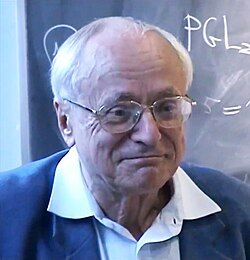
\includegraphics[width=1.80cm,height=2.20cm,keepaspectratio]{images/serre.jpg}
      };
      \node[inner sep=0pt] at (-2.8,0) {
        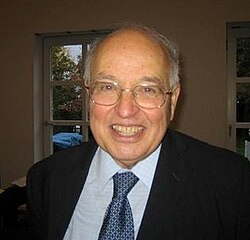
\includegraphics[width=1.80cm,height=2.20cm,keepaspectratio]{images/atiyah.jpg}
      };
      \node[inner sep=0pt] at (0.0,0) {
        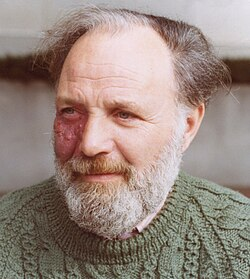
\includegraphics[width=1.80cm,height=2.20cm,keepaspectratio]{images/singer.jpg}
      };
      \node[inner sep=0pt] at (2.8,0) {
        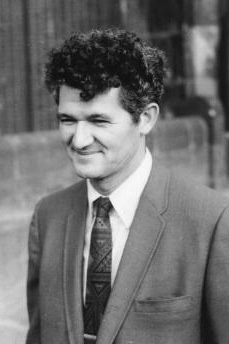
\includegraphics[width=1.80cm,height=2.20cm,keepaspectratio]{images/lax.jpg}
      };
      \node[inner sep=0pt] at (5.6,0) {
        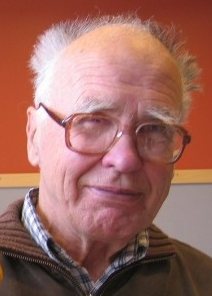
\includegraphics[width=1.80cm,height=2.20cm,keepaspectratio]{images/carleson.jpg}
      };
  \end{tikzpicture}}
\end{frame}

% Table slide 2: 2007–2010
\def\framesubject{群论·几何·概率}
\begin{frame}{2007–2010}
\vspace{-2pt}
\centering
\scriptsize
\begin{tabular}{@{}
  >{\raggedright}m{3.6cm}
  >{\centering}m{0.95cm}
  >{\centering}m{1.05cm}
  >{\raggedright}m{1.5cm}
  >{\raggedright}m{2.4cm}
  >{\raggedright\arraybackslash}m{2.6cm}
@{}}
\toprule
\rowcolor{abelbg}
\textbf{姓名} & \textbf{年份} & \textbf{生卒} & \textbf{国籍} & \textbf{机构} & \textbf{研究领域} \\
\midrule
\lrow{S. R. Srinivasa Varadhan\cn{斯里尼瓦瑟·瓦拉德汉}}{2007}{1940–}{印度/美国}{Courant Institute, NYU}{概率论、大偏差理论}
\lrow{John G. Thompson\fieldsbadge\wolfbadge\cn{约翰·汤普森}}{2008}{1932–}{美国}{Univ. of Florida}{群论；亦获 F1970 / W1992}
\lrow{Jacques Tits\wolfbadge\cn{雅克·蒂茨}}{2008}{1930–2021}{比利时/法国}{Collège de France}{群论、建筑理论；亦获 W1993}
\lrow{Mikhail Gromov\wolfbadge\cn{米哈伊尔·格罗莫夫}}{2009}{1943–}{俄罗斯/法国}{IHÉS}{几何；亦获 W1993}
\lrow{John Tate\wolfbadge\cn{约翰·泰特}}{2010}{1925–2019}{美国}{Univ. of Texas, Austin}{数论；亦获 W2002}
\bottomrule
\end{tabular}
\vspace{6pt}
  {\centering
  \begin{tikzpicture}
      \node[inner sep=0pt] at (-5.6,0) {
        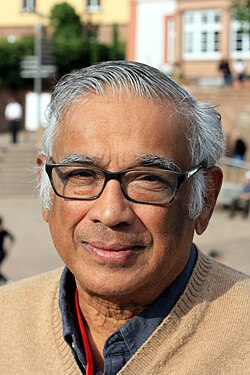
\includegraphics[width=1.80cm,height=2.20cm,keepaspectratio]{images/varadhan.jpg}
      };
      \node[inner sep=0pt] at (-2.8,0) {
        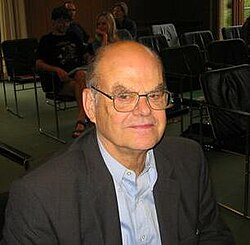
\includegraphics[width=1.80cm,height=2.20cm,keepaspectratio]{images/thompson.jpg}
      };
      \node[inner sep=0pt] at (0.0,0) {
        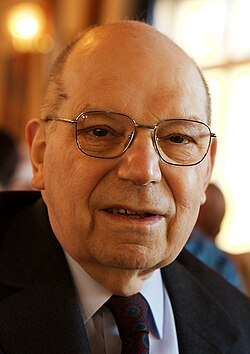
\includegraphics[width=1.80cm,height=2.20cm,keepaspectratio]{images/tits.jpg}
      };
      \node[inner sep=0pt] at (2.8,0) {
        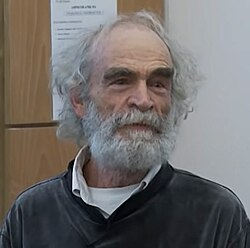
\includegraphics[width=1.80cm,height=2.20cm,keepaspectratio]{images/gromov.jpg}
      };
      \node[inner sep=0pt] at (5.6,0) {
        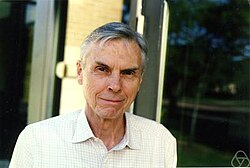
\includegraphics[width=1.80cm,height=2.20cm,keepaspectratio]{images/tate.jpg}
      };
  \end{tikzpicture}}
\end{frame}

% Table slide 3: 2011–2014
\def\framesubject{拓扑·组合·代数几何}
\begin{frame}{2011–2014}
\vspace{-2pt}
\centering
\scriptsize
\begin{tabular}{@{}
  >{\raggedright}m{3.6cm}
  >{\centering}m{0.95cm}
  >{\centering}m{1.05cm}
  >{\raggedright}m{1.5cm}
  >{\raggedright}m{2.4cm}
  >{\raggedright\arraybackslash}m{2.6cm}
@{}}
\toprule
\rowcolor{abelbg}
\textbf{姓名} & \textbf{年份} & \textbf{生卒} & \textbf{国籍} & \textbf{机构} & \textbf{研究领域} \\
\midrule
\lrow{John Milnor\fieldsbadge\wolfbadge\cn{约翰·米尔诺}}{2011}{1931–}{美国}{Stony Brook University}{拓扑、几何、代数；亦获 F1962 / W1989}
\lrow{Endre Szemerédi\cn{安德烈·塞迈雷迪}}{2012}{1940–}{匈牙利/美国}{Rényi Institute / Rutgers}{离散数学、理论计算机科学}
\lrow{Pierre Deligne\fieldsbadge\wolfbadge\cn{皮埃尔·德利涅}}{2013}{1944–}{比利时}{IAS Princeton}{代数几何；亦获 F1978 / W2008}
\lrow{Yakov Sinai\wolfbadge\cn{雅科夫·西奈}}{2014}{1935–}{俄罗斯/美国}{Princeton University}{动力系统、遍历论、数学物理；亦获 W1996}
\bottomrule
\end{tabular}
\vspace{6pt}
  {\centering
  \begin{tikzpicture}
      \node[inner sep=0pt] at (-5.2,0) {
        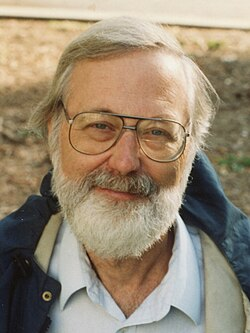
\includegraphics[width=1.80cm,height=2.20cm,keepaspectratio]{images/milnor.jpg}
      };
      \node[inner sep=0pt] at (-1.73,0) {
        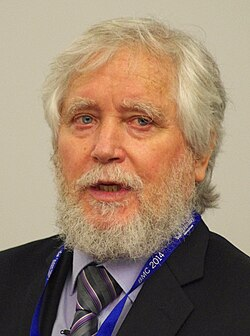
\includegraphics[width=1.80cm,height=2.20cm,keepaspectratio]{images/szemeredi.jpg}
      };
      \node[inner sep=0pt] at (1.73,0) {
        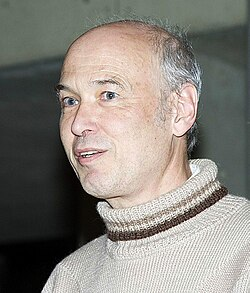
\includegraphics[width=1.80cm,height=2.20cm,keepaspectratio]{images/deligne.jpg}
      };
      \node[inner sep=0pt] at (5.2,0) {
        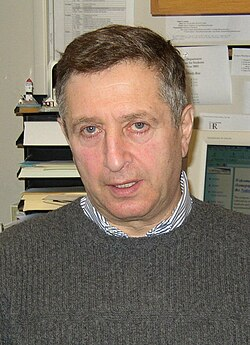
\includegraphics[width=1.80cm,height=2.20cm,keepaspectratio]{images/sinai.jpg}
      };
  \end{tikzpicture}}
\end{frame}

% Table slide 4: 2015–2018
\def\framesubject{偏微分方程·数论·小波}
\begin{frame}{2015–2018}
\vspace{-2pt}
\centering
\scriptsize
\begin{tabular}{@{}
  >{\raggedright}m{3.6cm}
  >{\centering}m{0.95cm}
  >{\centering}m{1.05cm}
  >{\raggedright}m{1.5cm}
  >{\raggedright}m{2.4cm}
  >{\raggedright\arraybackslash}m{2.6cm}
@{}}
\toprule
\rowcolor{abelbg}
\textbf{姓名} & \textbf{年份} & \textbf{生卒} & \textbf{国籍} & \textbf{机构} & \textbf{研究领域} \\
\midrule
\lrow{John F. Nash Jr.\nobelbadge\cn{约翰·纳什}}{2015}{1928–2015}{美国}{Princeton University}{非线性偏微分方程；亦获 N1994}
\lrow{Louis Nirenberg\chernbadge\cn{路易·尼伦伯格}}{2015}{1925–2020}{加拿大/美国}{Courant Institute, NYU}{非线性偏微分方程；亦获 C2010}
\lrow{Andrew Wiles\wolfbadge\cn{安德鲁·怀尔斯}}{2016}{1953–}{英国}{Univ. of Oxford}{数论、费马大定理；亦获 W1995}
\lrow{Yves Meyer\cn{伊夫·梅耶}}{2017}{1939–}{法国}{ENS Paris-Saclay}{小波分析}
\lrow{Robert Langlands\wolfbadge\cn{罗伯特·朗兰兹}}{2018}{1936–}{加拿大/美国}{IAS Princeton}{Langlands 纲领；亦获 W1995}
\bottomrule
\end{tabular}
\vspace{6pt}
  {\centering
  \begin{tikzpicture}
      \node[inner sep=0pt] at (-5.6,0) {
        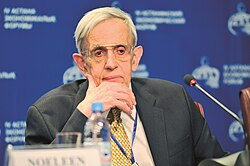
\includegraphics[width=1.80cm,height=2.20cm,keepaspectratio]{images/nash.jpg}
      };
      \node[inner sep=0pt] at (-2.8,0) {
        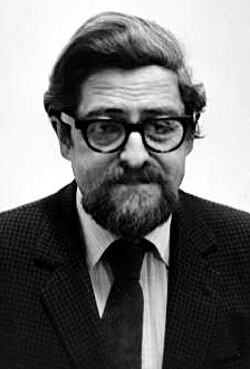
\includegraphics[width=1.80cm,height=2.20cm,keepaspectratio]{images/nirenberg.jpg}
      };
      \node[inner sep=0pt] at (0.0,0) {
        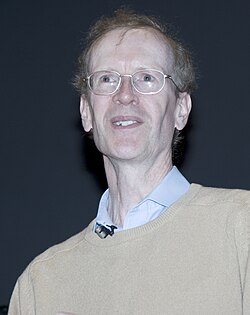
\includegraphics[width=1.80cm,height=2.20cm,keepaspectratio]{images/wiles.jpg}
      };
      \node[inner sep=0pt] at (2.8,0) {
        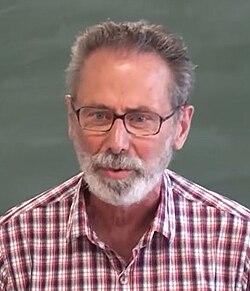
\includegraphics[width=1.80cm,height=2.20cm,keepaspectratio]{images/meyer.jpg}
      };
      \node[inner sep=0pt] at (5.6,0) {
        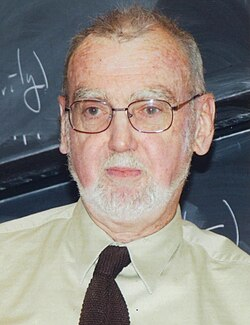
\includegraphics[width=1.80cm,height=2.20cm,keepaspectratio]{images/langlands.jpg}
      };
  \end{tikzpicture}}
\end{frame}

% Table slide 5: 2019–2021
\def\framesubject{几何分析·遍历论·理论计算机}
\begin{frame}{2019–2021}
\vspace{-2pt}
\centering
\scriptsize
\begin{tabular}{@{}
  >{\raggedright}m{3.6cm}
  >{\centering}m{0.95cm}
  >{\centering}m{1.05cm}
  >{\raggedright}m{1.5cm}
  >{\raggedright}m{2.4cm}
  >{\raggedright\arraybackslash}m{2.6cm}
@{}}
\toprule
\rowcolor{abelbg}
\textbf{姓名} & \textbf{年份} & \textbf{生卒} & \textbf{国籍} & \textbf{机构} & \textbf{研究领域} \\
\midrule
\lrow{Karen Uhlenbeck\cn{凯伦·乌伦贝克}}{2019}{1942–}{美国}{Univ. of Texas, Austin}{几何分析、规范场论；首位女性阿贝尔奖}
\lrow{Hillel Furstenberg\wolfbadge\cn{希勒尔·富斯滕伯格}}{2020}{1935–}{以色列/美国}{Hebrew Univ. of Jerusalem}{遍历论；亦获 W2006}
\lrow{Gregory Margulis\fieldsbadge\wolfbadge\cn{格里戈里·马尔古利斯}}{2020}{1946–}{俄罗斯/美国}{Yale University}{群论、遍历论；亦获 F1978 / W2005}
\lrow{László Lovász\wolfbadge\cn{拉斯洛·洛瓦兹}}{2021}{1948–}{匈牙利}{Eötvös Loránd Univ.}{理论计算机科学、离散数学；亦获 W1999}
\lrow{Avi Wigderson\turingbadge\cn{阿维·维格森}}{2021}{1956–}{以色列/美国}{IAS Princeton}{理论计算机科学；亦获 T2023}
\bottomrule
\end{tabular}
\vspace{6pt}
  {\centering
  \begin{tikzpicture}
      \node[inner sep=0pt] at (-5.6,0) {
        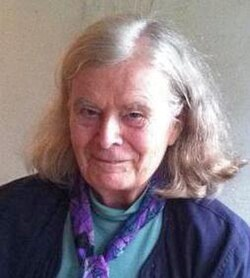
\includegraphics[width=1.80cm,height=2.20cm,keepaspectratio]{images/uhlenbeck.jpg}
      };
      \node[inner sep=0pt] at (-2.8,0) {
        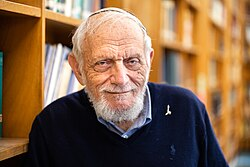
\includegraphics[width=1.80cm,height=2.20cm,keepaspectratio]{images/furstenberg.jpg}
      };
      \node[inner sep=0pt] at (0.0,0) {
        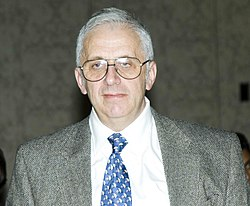
\includegraphics[width=1.80cm,height=2.20cm,keepaspectratio]{images/margulis.jpg}
      };
      \node[inner sep=0pt] at (2.8,0) {
        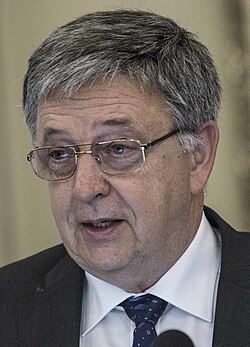
\includegraphics[width=1.80cm,height=2.20cm,keepaspectratio]{images/lovasz.jpg}
      };
      \node[inner sep=0pt] at (5.6,0) {
        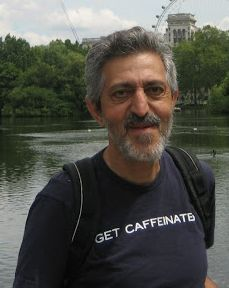
\includegraphics[width=1.80cm,height=2.20cm,keepaspectratio]{images/wigderson.jpg}
      };
  \end{tikzpicture}}
\end{frame}

% Table slide 6: 2022–2026
\def\framesubject{拓扑·PDE·概率·代数分析}
\begin{frame}{2022–2026}
\vspace{-2pt}
\centering
\scriptsize
\begin{tabular}{@{}
  >{\raggedright}m{3.6cm}
  >{\centering}m{0.95cm}
  >{\centering}m{1.05cm}
  >{\raggedright}m{1.5cm}
  >{\raggedright}m{2.4cm}
  >{\raggedright\arraybackslash}m{2.6cm}
@{}}
\toprule
\rowcolor{abelbg}
\textbf{姓名} & \textbf{年份} & \textbf{生卒} & \textbf{国籍} & \textbf{机构} & \textbf{研究领域} \\
\midrule
\lrow{Dennis Sullivan\wolfbadge\cn{丹尼斯·苏利文}}{2022}{1941–}{美国}{Stony Brook / CUNY}{拓扑、动力系统；亦获 W2010}
\lrow{Luis Caffarelli\wolfbadge\cn{路易斯·卡法雷利}}{2023}{1948–}{阿根廷/美国}{Univ. of Texas, Austin}{非线性偏微分方程、正则性理论；亦获 W2012}
\lrow{Michel Talagrand\cn{米歇尔·塔拉格朗}}{2024}{1952–}{法国}{CNRS Paris}{概率论、随机过程、泛函分析}
\lrow{Masaki Kashiwara\chernbadge\cn{柏原正树}}{2025}{1947–}{日本}{Kyoto University}{代数分析、表示论、D-模理论；亦获 C2018}
\lrow{Gerd Faltings\fieldsbadge\cn{格尔德·法尔廷斯}}{2026}{1954–}{德国}{Max Planck Institute, Bonn}{算术几何；亦获 F1986}
\bottomrule
\end{tabular}
\vspace{6pt}
  {\centering
  \begin{tikzpicture}
      \node[inner sep=0pt] at (-5.6,0) {
        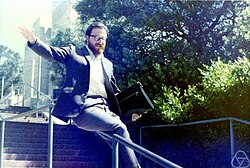
\includegraphics[width=1.80cm,height=2.20cm,keepaspectratio]{images/sullivan.jpg}
      };
      \node[inner sep=0pt] at (-2.8,0) {
        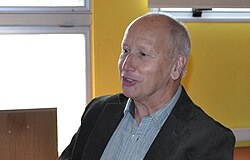
\includegraphics[width=1.80cm,height=2.20cm,keepaspectratio]{images/caffarelli.jpg}
      };
      \node[inner sep=0pt] at (0.0,0) {
        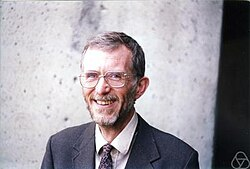
\includegraphics[width=1.80cm,height=2.20cm,keepaspectratio]{images/talagrand.jpg}
      };
      \node[inner sep=0pt] at (2.8,0) {
        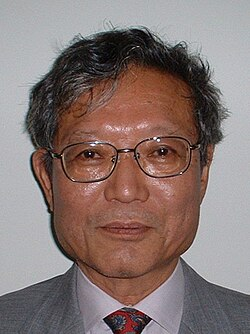
\includegraphics[width=1.80cm,height=2.20cm,keepaspectratio]{images/kashiwara.jpg}
      };
      \node[inner sep=0pt] at (5.6,0) {
        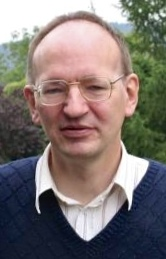
\includegraphics[width=1.80cm,height=2.20cm,keepaspectratio]{images/faltings.jpg}
      };
  \end{tikzpicture}}
\end{frame}

% Summary slide
\def\framesubject{菲尔兹·沃尔夫·陈省身·诺贝尔经济学·图灵奖交叉得主}
\begin{frame}{双料与大满贯}
\vspace{-4pt}
\centering
% --- Single tikzpicture for all 5 award rows + stats ---
\begin{tikzpicture}
  % Row 1: Fields — 7人 (Y top=0)
  \node[fill=fieldsclr, rounded corners=3pt, text width=2.8cm, minimum height=0.55cm,
        inner sep=0pt, align=center, anchor=north west] at (0,0)
    {\fontsize{6}{8}\selectfont\bfseries\color{white}$\blacklozenge$F\;\; 菲尔兹奖\;\; 7人};
  \node[anchor=north west, font=\fontsize{6}{8}\selectfont\bfseries, text=fieldsclr!70!black]
    at (3.05,0.00) {Serre\;·\;Atiyah\;·\;Thompson\;·\;Milnor\;·\;Deligne\;·\;Margulis\;·\;Faltings};

  % Row 2: Wolf — 17人 (Y top=-0.85)
  \node[fill=wolfclr, rounded corners=3pt, text width=2.8cm, minimum height=0.55cm,
        inner sep=0pt, align=center, anchor=north west] at (0,-0.85)
    {\fontsize{6}{8}\selectfont\bfseries\color{white}$\bigstar$W\;\; 沃尔夫奖\;\; 17人};
  \node[anchor=north west, font=\fontsize{6}{8}\selectfont\bfseries, text=wolfclr!65!black]
    at (3.05,-0.73) {Serre\;·\;Lax\;·\;Carleson\;·\;Thompson\;·\;Tits\;·\;Gromov\;·\;Tate\;·\;Milnor};
  \node[anchor=north west, font=\fontsize{6}{8}\selectfont\bfseries, text=wolfclr!65!black]
    at (3.05,-1.05) {Deligne\;·\;Sinai\;·\;Wiles\;·\;Langlands\;·\;Furstenberg\;·\;Margulis\;·\;Lovász\;·\;Sullivan\;·\;Caffarelli};

  % Row 3: Chern — 2人 (Y top=-1.70)
  \node[fill=chernclr, rounded corners=3pt, text width=2.8cm, minimum height=0.55cm,
        inner sep=0pt, align=center, anchor=north west] at (0,-1.70)
    {\fontsize{6}{8}\selectfont\bfseries\color{white}$\blacksquare$C\;\; 陈省身奖章\;\; 2人};
  \node[anchor=north west, font=\fontsize{6}{8}\selectfont\bfseries, text=chernclr!65!black]
    at (3.05,-1.72) {Nirenberg\;·\;Kashiwara};

  % Row 4: Nobel Economics — 1人 (Y top=-2.55)
  \node[fill=nobelclr, rounded corners=3pt, text width=2.8cm, minimum height=0.55cm,
        inner sep=0pt, align=center, anchor=north west] at (0,-2.55)
    {\fontsize{6}{8}\selectfont\bfseries\color{white}\faIcon{award}\;N\;\; 诺贝尔经济学奖\;\; 1人};
  \node[anchor=north west, font=\fontsize{6}{8}\selectfont\bfseries, text=nobelclr!65!black]
    at (3.05,-2.57) {John F. Nash Jr.\;(1994)};

  % Row 5: Turing — 1人 (Y top=-3.40)
  \node[fill=coverprimary, rounded corners=3pt, text width=2.8cm, minimum height=0.55cm,
        inner sep=0pt, align=center, anchor=north west] at (0,-3.40)
    {\fontsize{6}{8}\selectfont\bfseries\color{white}\faIcon{desktop}\;T\;\; 图灵奖\;\; 1人};
  \node[anchor=north west, font=\fontsize{6}{8}\selectfont\bfseries, text=coverprimary!65!black]
    at (3.05,-3.42) {Avi Wigderson\;(2023)};

  % Separator line
  \draw[mutedgray!40, line width=0.4pt] (0,-4.10) -- (\textwidth,-4.10);

  % Stats bar
  \fill[abelbg, rounded corners=4pt] (0,-4.35) rectangle (\textwidth,-5.10);
  \node[anchor=north, font=\fontsize{5.5}{7}\selectfont\bfseries, text=abelclr]
    at (0.17\textwidth,-4.47) {首届\;\; Jean-Pierre Serre\;(2003)};
  \node[anchor=north, font=\fontsize{5.5}{7}\selectfont\bfseries, text=abelclr]
    at (0.50\textwidth,-4.47) {首位女性\;\; Karen Uhlenbeck\;(2019)};
  \node[anchor=north, font=\fontsize{5.5}{7}\selectfont\bfseries, text=abelclr]
    at (0.85\textwidth,-4.47) {$\blacklozenge$F+$\bigstar$W+A\;\; Serre\;·\;Milnor\;·\;Deligne\;·\;Margulis};
  \draw[abelclr!30, line width=0.4pt] (0.37\textwidth,-4.40) -- (0.37\textwidth,-5.05);
  \draw[abelclr!30, line width=0.4pt] (0.68\textwidth,-4.40) -- (0.68\textwidth,-5.05);\end{tikzpicture}
\end{frame}


\end{document}
